\documentclass[spanish,12pt]{article}
\usepackage[spanish]{babel}
\usepackage[utf8]{inputenc}
\usepackage{xspace}
\usepackage{lmodern}
\usepackage{indentfirst}
\usepackage{xargs}
\usepackage{ifthen}
\usepackage{fancyhdr}
\usepackage{latexsym}
\usepackage{lastpage}
\usepackage{textcomp}
\usepackage{varwidth}
\usepackage{caratula, aed2-tad,aed2-symb,aed2-itef}
\usepackage{algorithmicx, algpseudocode, algorithm}
\usepackage{enumerate}
\usepackage{graphicx}
\usepackage{caption}
\usepackage{subcaption}
\usepackage{float}
\usepackage{anysize}
\marginsize{1.5cm}{1.5cm}{1.5cm}{1.5cm}

\begin{document}

\titulo{Informe 1}
\materia{Algoritmos y Estructuras de Datos III}
\author{Grupo  \\Alvarez Vico Jazm\'in\\Cortés Conde Titó Javier María\\Pedraza Marcelo \\ Rozenberg Uriel Jonathan}

\integrante {Jazmín Alvazer Vico}{75/15}{jazminalvarezvico@gmail.com}
\integrante {Marcelo Pedraza}{393/14}{marcelopedraza314@gmail.com}
\integrante {Uriel Jonathan Rozenberg}{838/12}{rozenberguriel@gmail.com}
\integrante {Javier María Cortés Conde Titó}{252/15}{javiercortescondetito@gmail.com}

\maketitle


\clearpage

\tableofcontents
\cleardoublepage

\section{Problema 1: Cruzando el puente}

\subsection{Introducción}

En este problema, un grupo formado por arquéologos y caníbales debe cruzar un puente. El mismo sólo puede ser atravesado por dos personas a la vez, y tiene que ser cruzado con una linterna. Como el grupo sólo dispone de una linterna, siempre debe regresar alguno al lado del puente original. Además, en ningún lado del puente puede haber más caníbales que arquéologos.
Cada individuo consta de la propiedad ´´velocidad", un número natural que indica cuánto tiempo tarda en atravesar el puente. Si dos personas atraviesan el puente juntas, lo hacen en el tiempo más grande entre los dos.
Formalmente queremos encontrar la solución óptima para minimizar el tiempo que toma atravesar un trayecto por dos conjuntos de individuos cuando uno de ellos no puede ser mayor al otro(exceptuando el caso en que uno de ellos es vacío).

\subsection{Explicación de la solución}
Para resolver este problema, usamos la técnica de backtracking: utilizamos una función recursiva para poder probar todos los caminos posibles que no generen situaciones en las cuales hay mas caníbales que arqueólogos en algún lado del puente. Finalmente elegímos el mínimo de los subcaminos recorridos.

Para empezar, todos los casos donde ya se comience de un lado del puente con más caníbales que arqueólogos no tienen solución.
El caso en el cual no haya arquéologos usamos una instancia aparte que conlleva muchas condiciones booleanas. Este caso se resuelve simplemente utilizando al caníbal más rápido para llevar a los demás. Para ver que esto es óptimo, basta ver que todos los individuos deben pasar al menos una vez. Para cualquier ida y vuelta la linterna, que vaya y vuelva el caníbal más rápido genera el mismo estado que cualquier otra opción, con un menor ´´costo".


Para los demás casos hay que analizar los cinco ´´movimientos"  válidos existentes para atravesar el puente: Pasar dos caníbales, dos pasar arqueólogos,pasar sólo un arqueólogo, pasar sólo un canibal o pasar un arqueólogo y un caníbal.
Decidimos pensar la ida y vuelta de la linterna como un sólo estado, para no tener que registrar la ubicación de la misma.
Para guardar la información de posiciones vamos a registrar el estado del lado izquierdo(o inicial) del puente, ya que cualquier individuo que no esté de ese lado, necesariamente estará del otro. Utilizamos una matriz de dimensión N+1xM+1 y cuatro listas($N_A$ y $M_A$ para indicar quiénes estan en el punto de partida y $N_B$ y$ M_B$ para el punto de llegada). Cada vez que modifiquemos $N_A$ y $M_B$ se entrará en la recursión copiando la matriz y registrando en la misma el nuevo estado recorrido.
Todos los resultados posibles se guardan en una lista para poder finalmente devolver el valor minimo de la misma el cual será nuestra solución.
La función PuedenSalir verifica que, en caso de que cruzen el puente los individuos indicados, no generará problemas en ninguno de los lados del puente.



\subsection{Pseudocódigo}

A lo largo de esta sección renombraremos tipos, para facilitar la lectura.
\begin{itemize}
	\item vint es un arreglo de enteros.
	\item ins es una dupla (vint, vint).
	\item instancias es un conjunto de ins.
\end{itemize}
\\
Tambien nos ahorraremos algunos pseudocódigos que son casos análogos entre Arqueólogos y caníbales.

\begin{algorithm}[H]{\textbf{BT}() }
	\begin{algorithmic}
<<<<<<< HEAD
		\If{$N_A$ es vacía}
			\State min $\gets$  mínimo de $M_A$
			\State devolver min*($|M_B|-1$)+ Sumatoria( $M_B$ sin el elemento min)
		\EndIf
		\State M[$|N_A$|+1][$|M_A|$+1] $\gets$1
		\State T $\gets$ []

		\While{i= 0,1,2}
			\While{j= 0,..,2-i}
				\If{¬(i$\eq$j$\eq$0) PuedenSalir(i,j,$|N_A|,|M_A|,|N_{B}|,|M_{B}|$)}
					\State se le quitan i elementos a $N_A$ y se le agregan a $N_B$
					\State se le quitan j elementos a $M_A$ y se le agregan a $M_B$
					\State (si i,j=1 se quita el más rápido, si i,j=2 se quitan el más rápido y el más lento)
					\State t $\gets$ Max(de los elementos transferidos)
					\While{k=0; k$\leq$2; k++}
						\While{l=0; k+l$\leq$2; l++}
							\If{PuedenSalir(k,l,$|N_A|,|M_A|,|N_{B}|,|M_{B}|$) $\land$ M[$N_A$+k][$M_A$+l]=0} %verificar esto
								\State se le quitan k elementos a $N_B$ y se le agregan a $N_A$
								\State se le quitan l elementos a $M_B$ y se le agregan a $M_A$
								\State (se quitan los dos más rápidos)
								\State t=t+Max(de los elementos transferidos)+ BT(M,$N_A,M_A,N_B,M_B$)
								\State T.Agrergar(t)
							\EndIf
						\EndWhile
					\EndWhile
				\EndIf
			\EndWhile $//O(1)$
		\EndWhile$//O(Log(P))$
		\State devolver Min(T)
=======
		\State Para todo arqueologo en el lado A
		\State \quad  velArq=velocidad del aqueologo
		\State \quad muevo arqueologo al lado B
		\State \quad voyConA(velArq)
		\State \quad voyConC(velArq)
		\State \quad vuelvo al arqueologo al lado A
		\State fin para
		\State para todo canibal en el lado A
		\State \quad velCan = velocidad del Canibal
		\State \quad muevo al canibal al lado B
		\State \quad voyConC(velArq)
		\State \quad  vuelvo el canibal al lado A
		\State fin para
	\end{algorithmic}
\end{algorithm}
>>>>>>> 4a8425857147caa501c99d4c34ee083170f1f32f

\begin{algorithm}[H]{\textbf{voyConA}(int valElem1)}
	\begin{algorithmic}
	\State Para todo arqueologo en A
	\State \qquad valElem $\gets$ velocidad del arqueologo
	\State \qquad maximo $\gets$ max(valElem, velElem1)
	\State \qquad mMinActual $\gets$ mMinActual + maximo
	\State \qquad muevo al aqueologo al lado B
	\State \qquad VuelvoCon()
	\State \qquad mMinActual $\gets$ mMinActual - maximo
	\State \qquad vuelvo al arqueologo al lado A	
	\State finPara
	\end{algorithmic}
\end{algorithm}

\begin{algorithm}[H]{\textbf{voyConC}(int valElem1)}
	\begin{algorithmic}
		\State  analogo a voyConA pero en lugar de arqueologos utilizamos canibales
	\end{algorithmic}
\end{algorithm}
 	
\begin{algorithm}[H]{\textbf{esValida}(instancia: ins) $\to$ $res$ : bool }
	\begin{algorithmic}
	 res $\gets$ (cantidad de arqueologos de un lado$\geq$ cantidad de canibales del mismo lado) $\lor$ cantidad de arqueologos del lado es 0)
	\end{algorithmic}
\end{algorithm}


\begin{algorithm}[H]{\textbf{vuelvoCon}(\textbf{InOut} mMinActual:Nat, \textbf{InOut} mMinimoGlobal:Nat, \textbf{InOut} ArqA: vint, \textbf{InOut} ArqB: vint), \textbf{InOut} canA: vint, \textbf{InOut} canB: vint), \textbf{InOut} MIsntanciasSet: instancias}
	\begin{algorithmic}
	\State Sí no esValida(lado A) o no esValida(lado B)	
	\State \quad Interrumpi
	\State finSi
	\State Sí la cantidad de arqueologos en A es cero y la cantidad de canibales en A es cero
	\State \quad Sí mMinActual < mMinimoGlobal
	\State \qquad mMinimoGlobal $\gets$ mMinActual
	\State \quad finSi
	\State  \quad Interrumpi
	\State finSi
	\State Para todo arqueologo en B 
	\State \qquad valElem $\gets$ velocidad del arqueologo
	\State \qquad mando al arqueologo al lado A	
	\State \qquad Sí esta instancia no esta en instancias
	\State \qquad \quad mMinActual $\gets$ mMinActual + valElem
	\State \qquad \quad instancias $\cup$ \{ instancia \}
	\State \qquad \quad BT()
	\State \qquad \quad instancias - \{ instancia \}
	\State \qquad \quad mMinActual $\gets$ mMinActual - valElem
	\State \qquad finSi
	\State \qquad vuelvo al arqueologo al lado B
	\State \quad finSi
	\State finPara
	\State ParaTodo canibal en B
	\State \quad \textbf{if}(canB[i] > 0)
	\State \qquad analogo al for anterior pero con canibales
	\State finPara
	\State Para Todo arqueologo en B 
	\State \quad valElemArq $\gets$ velocidad del arqueologo 
	\State \qquad mando al arqueologo al lado A
	\State \qquad Para todo canibal en B
	\State \qquad \quad valElemCan $\gets$ velocidad del canibal	
	\State \qquad \qquad mando al canibal al lado A
	\State \qquad \qquad Si esta nueva instancia no esta en instancias
	\State \qquad \qquad \quad max $\gets$ Maximo(valElemArq, valElemCan)
	\State \qquad \qquad \quad mMinAcutal $\gets$ mMinActual + max
	\State \qquad \qquad \quad BT()
	\State \qquad \qquad \quad instancias - \{ instancia \}
	\State \qquad \qquad \quad mMinActual $\gets$ mMinActual - maximo
	\State \qquad \qquad finSi
	\State \qquad \qquad vuelvo al canibal al lado B
	\State \qquad vuelvo al aqueologo al lado B 
	\State \qquad finPara
	\State finPara
																		
	\end{algorithmic}
\end{algorithm}
 $//O(1)$
 $//O(1)$
\subsecti on{Demostración de Correctitud}

Para mostrar la correctitud de nuestro algoritmo queremos ver dos cosas:
\begin{itemize}

	\item Recorre todos los casos: \\
Si planteamos nuestras posibilidades como una matríz, vemos que todo lo pertinente al triángulo superior no tiene solución de manera trivial o se plantea un caso particular; estos casos son: los que hay sólo caníbales, o hay más caníbales que arquéologos desde un comienzo. Entonces nos concentraremos en el triángulo inferior.
Al ser nuestro algoritmo una función recursiva solo terminará al llegar al caso base. Podemos ver que nuestro caso base se alcanza al obtener las dos listas inciales($N_A$, $M_A$) vacías.
Como vemos en el primer conjunto de for, creamos  tuplas (i,j) tal que generan todas las posibles formas de pasar el puente, si esa tupla puede realmente pasar por el puente, se crea una copia de las listas $N_A$, $M_A$, $N_B$, $M_B$ donde, dependiendo del i, se sacan esa cantidad de elementos la lista $N_A$ y se ponen en $N_B$ caso análogo con j y $M$'s.
Al generar todas las instancias del cruce del puente, ahora tenemos que saber todas las formas de volver el puente. De una forma similar a la explicada antes los últimos dos whiles funcionan tal que generan todas las formas de volver del puente.

	\item No hace ciclos: \\
Nuestro algoritmo no admite ciclos puesto que tiene una condición booleana sobre la matriz, la cual no permite volver a una instancia anterior en las que esté el mismo conjunto de caníbales y arquéologos que en los casos anteriores. La misma consiste en que sólo pueden regrsar los individuos si y sólo si en la posición (i,j) (donde $i= N_A$+(los arquéologos que regresen) y $j=M_A$ + (los caníbales que regresan) ) hay un cero. Cada vez que se llama a la función recursivamente la posición inicial en el punto A es marcada con un 1. De esta forma es imposible realizar ciclos.

\end{itemize}




\subsection{Demostración de Complejidad}
	Si pensamos todas nuestras posibilidades como un árbol de estados, haciendo que la función ´´ida" y ´´vuelta" genera 3 hijos y 4 hijos respectivamente(la función ´´vuelta" genera 5 hijos, pero uno de ellos es siempre un estado por el que ya pasamos).
	 Además, la altura nunca va a ser mayor que $n*m/2$, ya que tenemos una matriz para verificar que no pasemos dos veces por el mismo estado. Además, las operaciones de cada estado consisten en ´´recorrer" todas las posibilidades de individuos a mandar, siendo esto %%VER BIEN ESTO
	 En resumen, la cantidad máxima de resultados es altura del árbol por la ´´amplitud": Podemos ver que la complejidad es $12^{n*m/2}$
\subsection{Experimentación}
Para este problema generamos dos hipótesis:
Suponemos que siempre que van dos individuos, si son del mismo tipo van los dos extremos(el más lento y el más rapido) y si son distinto tipo, pasa el mínimo de todo el grupo, y el máximo del otro tipo.
En el caso de la vuelta, siempre se vuelve con los más veloces posibles.
Queremos ver si esta estrategia sigue dando resultados óptimos, y cuál es la relación de complejidad
\\
Por otro lado, suponemos que el conjunto particular de caníbales y arquéologos en un lado de puente es indistinguible en los estados, y que alcanza con contemplar la cantidad. Es decir, si la hipótesis anterior se cumple, no sería necesario probar cada conjunto particular, reduciendo considerablemente la complejidad.



\section{Problema 2: Problemas en el camino}

\subsection{Introducción}

En el problema enunciado, Nuestros exploradores se encuentran con una balanza de dos platos; en el de la izquierda la llave que necesitan. Para que esta sea de utilidad, al tomarla deben mantener el equilibrio de la balanza, y para realizar esto cuentan con pesas de peso igual a las potencias de tres (una pesa por potencia).
Sabiendo el peso de la llave, necesitamos saber qué pesas poner en cada plato para mantener el equilibrio original.
Podemos pensar que el lado derecho de la balanza equivale a la operación de sustracción y el izquiero a la adición. De esta forma, al agregar pesas de un lado o del otro estaríamos sumando o restando su peso.
Esto equivale a decir que, dado un entero P queremos componerlo en sumas y restas de potencias de tres distintas.

\subsection{Explicación de la solución}

Para resolver este problema, Reescribimos P en la base ternaria, y a esta secuencia la notaremos T. Entonces tenemos $P = \sum_{i=0}^{n} a_i3^i$  con $0 \leq a_i \leq 2$ y $n = log_{3}{(P)}$  entonces $T ={a_1,a_2,...,a_n}$.
Luego, tomamos en orden creciente los elementos de T. Si $a_i$ es 0, no hacemos nada. Si $a_i$ es 1, en la balanza izquierda colocamos la pesa que corresponde a $3^i$. Si $a_i =2$, colocamos una pesa de $3^i$ en la balanza derecha y sumamos 1 a $a_{(i+1)}$ (y consecuentemente, se cambian los valores posteriores de T para que continúe en base ternaria)


\subsubsection{Pseudocódigo}

Nota: Para la implementación, en vez de crear el conjunto T, vamos tomando el resto de P y dividiéndolo por 3. Entonces, el valor de la variable ´´rem" sería el equivalente al $a_i$ (i responde al número de iteraciones ya hechas)

\begin{algorithm}[H]{\textbf{Pesas}(Natural: P)}
	\begin{algorithmic}[1]
		\State pesa $\gets$ 1 $//O(1)$
		\While{ P $>$ 0}$//O(Log(P))$
		 	\State rem $\gets$ $r_3 (P)$ $//O(1)$
	    		\State P $\gets $ parte entera(P/3) $//O(1)$
	    		\If{rem = 1} $//O(1)$
	    			\State pesa va para la balanza izquierda     $//O(1)$    			\Else
				\If{ rem = 2} $//O(1)$
	    				\State p$\gets$ P+1   $//O(1)$
	    				\State pesa va para la balanza derecha  $//O(1)$
				\EndIf
			\EndIf
			\State pesa $\gets$ pesa*3  $//O(1)$
		\EndWhile
	\end{algorithmic}
\end{algorithm}



\subsubsection{Demostración de Correctitud}

Primero probaremos dos lemas:
$\forall n \in N$ vale que  $2*3^{n} = 3^{n+1}-3^{n}$.

lema 1:$ 2*3^{n} = 3^{n+1}-3^{n} \Longleftrightarrow 2*3^{n}+3^{n} = 3^{n+1} \Longleftrightarrow (2+1)*3^{n} = 3^{n+1} \Longleftrightarrow   3*3^{n} = 3^{n+1} \Longleftrightarrow  3^{n+1} = 3^{n+1}$ 

lema2 : probaremos por inducción que $ \Sum_{0}^{n}{3^{i}} < 3^{n+1}$
caso base: $n \eq 0$. $3^{0} < 3^{1}$
Paso Inductivo: 
	Supongo que $ \Sum_{0}^{n}{3^{i}} < 3^{n+1}$
	Quiero ver que $ \Sum_{0}^{n+1}{3^{i}} < 3^{n+2}$
	$ \Sum_{0}^{n+1}{3^{i}} \eq \Sum_{0}^{n}{3^{i}} + 3^{n+1}$
	por Hipótesis Inductiva, $\Sum_{0}^{n}{3^{i}} + 3^{n+1} < 3^{n+1} + 3^{n+1} < 3^{n+2} $
\\
Ahora para probar la correctitud del algoritmo, desarrollaremos algunos conceptos algebraicos.
Por el algoritmo de división de Euclides sabemos que podemos escribir \\  $P= q*3+ r_{3}(P)$ con $0\leq r_{3}(P) \leq 2 $. Luego, podemos escribir $q= z*3 + r_{3}(q)$, entonces $P= (z*3 + r_{3}(q))*3 +r_{3}(P)$ y así recursivamente y aplicando la distributividad de la suma podemos descomponer p en las potencias de 3. Finalmente obtendríamos $p= \sum_{i=0}^{n}{a_i 3^{i}} $ con $0 \leq a_i \leq 2$.

Ahora nuestro problema es la aparición de $a_i=2$ en la descomposición, puesto que sólo tenemos una pesa por potencia de tres.

Probaremos por inducción global  que dado un natural P y su representación en potencias de dos $a_{i}$, $ \forall n \in N vale  \sum_{0}^{n}{a_{i}*3^{i}}= \sum_{0}^{n+1}{b_{i}*3^{i}} con 0\leq a_{i} \leq 2 y -1 \leq b_{i} \leq 1$. Podemos ver que $b_{n+1}\neq -1$, ya que P esto generaría un número negativo, y p es natural.

caso base:  
$\sum_{0}^{n}{a_{i}*3^{i}}= \sum_{0}^{n+1}{b_{i}*3^{i}} con 0\leq a_{i} \leq 2 y -1 \leq b_{i} \leq 1$
Existen tres opciones. En el caso que $a_{0} \eq 0$, $b_{0} \eq 0$ y $b_{1} \eq 0$.
En el caso $a_{0} \eq 1$, $b_{0} \eq 1$ y $b_{1} \eq 0$.
Finalmente, en el caso $a_{0} \eq 2$, usamos el lema 1, lo que nos da $b_{0} \eq -1$ y $b_{1} \eq 1$

paso inductivo:
 supongo que $\sum_{0}^{n}{a_{i}*3^{i}} \eq \sum_{0}^{n+1}{b_{i}*3^{i}} con 0\leq a_{i} \leq 2 y -1 \leq b_{i} \leq 1$
 quiero ver que $\sum_{0}^{n+1}{a_{i}*3^{i}}= \sum_{0}^{n+2}{b_{i}*3^{i}} con 0\leq a_{i} \leq 2 y -1 \leq b_{i} \leq 1$
\\
$\sum_{0}^{n+1}{a_{i}*3^{i}} \eq \sum_{0}^{n}{a_{i}*3^{i}} + a_{n+1}*3^{n+1}$
Por Hipótesis Inductiva, $ \sum_{0}^{n}{a_{i}*3^{i}} + a_{n+1}*3^{n+1} \eq \sum_{0}^{n+1}{b_{i}*3^{i}} + a_{n+1}*3^{n+1} \eq \sum_{0}^{n}{b_{i}*3^{i}} + a_{n+1}*3^{n+1} + b_{n+1}*3^{n+1} $
Observemos $a_{n+1} + b_{n+1}$. Esta suma puede dar $0,1,2,3$.
El caso 0 y 1 son triviales. Basta llamar al nuevo $b_{n+1}$ a la suma y $b_{n+2} \eq 0$
El caso 3, $b_{n+1}$ pasa a ser 0, y $b_{n+2}$ pasa a ser 1
En el caso 2, por lema 1 podemos decir que $b_{n+1}$ pasa a ser -1, y $b_{n+2}$ pasa a ser 1.



%viejo%

$p= \sum_{i=0}^{n}{a_i 3^{i}} =  \sum_{i=0}^{n-1}{a_i 3^{i}} + a_n*3^{n}$ 

por hipotesis inductiva, sabemos que para $0\leq i \leq n-1, -1\leq a_{i}\leq 1$. Por Euclides, como explicamos antes, $0\leq a_{n} \leq 2 $ en los primeros dos casos es trivial la validez de la proposición. 
Veamos el caso a_{i} = 2:
  Por el lema, podemos escribir $2*3^{n}= = 3^{n+1}-3^{n}$  entonces  podemos escribir a_{i} p= \sum_{i=0}^{n}{a_i 3^{i}} = \sum_{ 


 Pero por lo visto en el lema anterior, $2*3^{i}= 3^{i+1}-3^{i}$. Esto equivale a colocar la pesa $3^{i+1}$ en la balaza izquierda y la $3^{i}$ en la derecha, obteniendo el equivalente a 2 pesas $3^{1}$ en la izquierda. aplicando este proceso recursivamente, obtenemos  una descomposición de P sumando y restando sus potencias de tres sin repeticiones.


\subsubsection{Demostración de Complejidad}

<<<<<<< HEAD
%El algoritmo consta de un ciclo, dentro de cada iteración, se calcula el resto y hace dos comparaciones; todas estas operaciones se ejecutan en O(1), mientras que colocar la pesa en cada balanza
%es agregar un número al final de una lista. Como el modelo de lista que usamos es ´´List", esto se realiza en $\mathcal{O}(1)$.
%Entonces, dentro de cada iteración solo se hacen operaciones en $\mathcal{O}(1)$. Esto hace que la complejidad sea la cantidad de iteraciones que hace el ciclo.
%
%Si nos abstraemos del if, el ciclo tiene como condición que P$>$0, siendo P el valor de entrada. Como podemos observar, P es modificado dividiéndose por 3 cada iteración. Por álgebra básica sabemos que se necesesitarán como mucho $log_3(P) + 1$ iteraciones para que P sea menor a 0.
%Ahora, tomando en cuenta el if hay un caso en el cual le sumamos 1 a P, lo cual afecta un poco la cuenta; volvemos a la explicación del algoritmo y tomamos el conjunto $T = {a_1,...,a_n}$
%donde  $P = \sum_{i=0}^{n} a_i3^i$ con $0 \leq a_i \leq 2$ y $n = log_{3}{P}$, siendo el valor de rem el valor de $a_i$ en la iésima iteración.
%Cuando hacemos que $P<-P+1$ nos queda que en la próxima iteración rem valdría uno más, es decir $a_{i+1}$ pasaría a valer uno más de lo que valdría en T. Ahora,  siendo estos que para todo $a_k$
%valen entre 0 y 2, si $a_{i+1}$ en vez de valer 3, valdría 0 y $a_{i+2}$ valdría uno más también, y si  $a_{i+2}$ valía 2, pasaría a valer 0 y  $a_{i+3}$ valdría uno más, y así sucesivamente hasta llegar a $a_n$.
%Y si resulta que también $a_n$ valía 2, entonces tendríamos un $a_{n+1}$ que pasaría a valer 1 y $a_n$ valdría 0.
%Luego no hay mas casos donde $a_j$ (para $i<j<=n$) sea 2, entonces no hay más casos donde puedan volver a ocurrir este tipo de cosas, quedándonos asi, un máximo de $Log_3(P)+1$ iteraciones.
%
%Entonces, la complejidad del algoritmo es de $\mathcal{O}(Log_{3}(P))$.
%Luego, se puede probar que Log(P) es $\mathcal{O}(\sqrt(P))$
=======
El algoritmo consta de un ciclo, dentro de cada iteración, se calcula el resto y hace dos comparaciones; todas estas operaciones se ejecutan en O(1), mientras que colocar la pesa en cada balanza
es agregar un número al final de una lista. Como el modelo de lista que usamos es ´´List", esto se realiza en $\mathcal{O}(1)$.
Entonces, dentro de cada iteración solo se hacen operaciones en $\mathcal{O}(1)$. Esto hace que la complejidad sea la cantidad de iteraciones que hace el ciclo.


Podemos ver en el pseudocódigo que sólo se incrementa a P cuando es congruente a 2 módulo 3. En caso contrario, es fácil ver que la complejidad es de $\mathcal{O}(Log_{3}(P))$, ya que en cada iteración se divide a P por 3, quedándose con la parte entera.
Supongamos el caso en el cual, para cada iteración, a P se la divide por 3, se calcula la parte entera y se le incrementa 1(es decir, siempre se entra en la condición $rem \eq 2$). Se puede ver que ese incremento no genera un cambio en el orden de complejidad
Entonces, la complejidad del algoritmo es de $\mathcal{O}(Log_{3}(P))$.
Luego, se puede probar que Log(P) es $\mathcal{O}(\sqrt(P))$
>>>>>>> 07e1e05216c3d0cd0569c50823acb3bc96dfe0d3




%%Explicacion vieja

% Si nos abstraemos del if, el ciclo tiene como condición que P$>$0, siendo P el valor de entrada. Como podemos observar, P es modificado dividiéndose por 3 cada iteración. Por álgebra básica sabemos que se necesesitarán como mucho $log_3(P) + 1$ iteraciones para que P sea menor a 0.
% Ahora, tomando en cuenta el if hay un caso en el cual le sumamos 1 a P, lo cual afecta un poco la cuenta; volvemos a la explicación del algoritmo y tomamos el conjunto $T = {a_1,...,a_n}$ 
% donde  $P = \sum_{i=0}^{n} a_i3^i$ con $0 \leq a_i \leq 2$ y $n = log_{3}{P}$, siendo el valor de rem el valor de $a_i$ en la iésima iteración.
% Cuando hacemos que $P<-P+1$ nos queda que en la próxima iteración rem valdría uno más, es decir $a_{i+1}$ pasaría a valer uno más de lo que valdría en T. Ahora,  siendo estos que para todo $a_k$
% valen entre 0 y 2, si $a_{i+1}$ en vez de valer 3, valdría 0 y $a_{i+2}$ valdría uno más también, y si  $a_{i+2}$ valía 2, pasaría a valer 0 y  $a_{i+3}$ valdría uno más, y así sucesivamente hasta llegar a $a_n$.
% Y si resulta que también $a_n$ valía 2, entonces tendríamos un $a_{n+1}$ que pasaría a valer 1 y $a_n$ valdría 0.
% Luego no hay mas casos donde $a_j$ (para $i<j<=n$) sea 2, entonces no hay más casos donde puedan volver a ocurrir este tipo de cosas, quedándonos asi, un máximo de $Log_3(P)+1$ iteraciones.

% Entonces, la complejidad del algoritmo es de $\mathcal{O}(Log_{3}(P))$.
% Luego, se puede probar que Log(P) es $\mathcal{O}(\sqrt(P))$


\subsection{Experimentación}
 Al momento de la experimentación inicialmente teníamos la idea de que, al no tener mejores ni peores casos a nivel de complejidad teórica, no importaba mucho que valores de P que se ingresaban, e iba a ser siempre creciente.

\subsubsection{Análisis complejidad te\'orica}
 Para el análisis de la complejidad te\'orica decidimos simplemente medir los tiempos del algoritmo aumentando el valor de entrada desde 1 hasta la cota puesta por el enunciado.
  Después de observar los resultados, encontramos una función O(Log(n)) que se asemeje aproximadamente a los resultados de las mediciones del algoritmo para poder compararlo.
  Terminamos usando la funcion $500*log_3(x)$.
  Notamos que no quedaba muy claro cómo es que las mediciones se asemejaban a $log_3(x)$. Entonces decidimos cambiar la escala:
  En vez de presentar un gráfico que muestre los ejes (X,Y) = (peso de la llave, mediciones) lo vamos a mostrar como (X,Y) = (Log(peso de la llave),Log(mediciones))

	\begin{figure}[H]
	\centering
	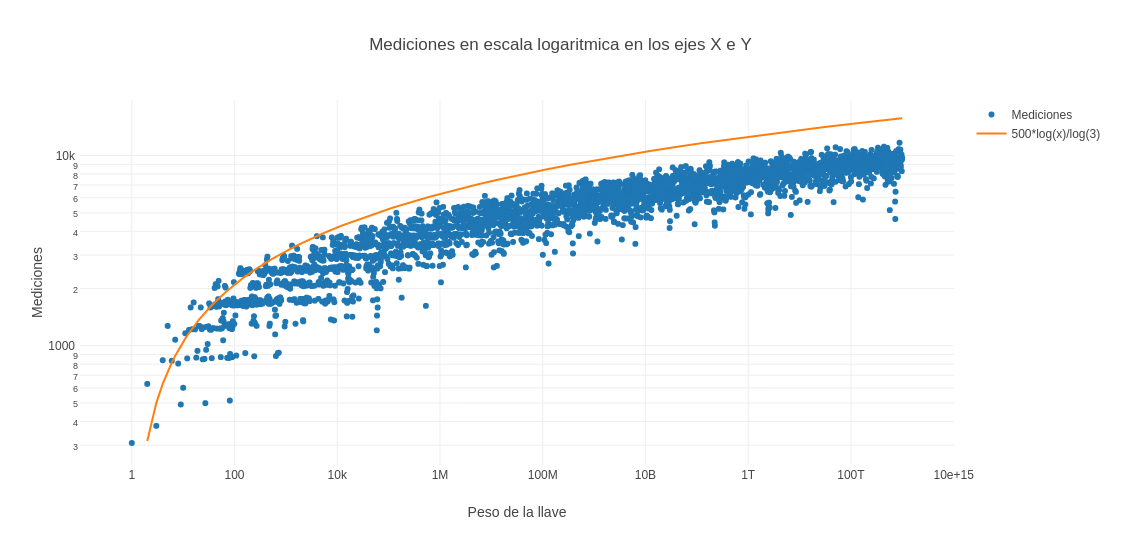
\includegraphics[width=0.8\textwidth]{punto2-mediciones}
	\caption{Mediciones de la implementaci\'on comparado con $500*log_{3}{n}$ en escala logaritmica en X e Y}
	\end{figure}



\subsubsection{Análisis}
Luego realizado el gráfico notamos que, a pesar de de que las mediciones simulaban cumplir las condiciones de la complejidad, esperábamos un comportamiento más cercano a que vaya aumentando en rectas horizontales, ya que se hacía la misma cantidad de iteraciones para cada valor del logaritmo en base 3. Pero en vez de eso éstas tenían un tipo de patrón ligeramente distinto.

\begin{figure}[H]
\centering
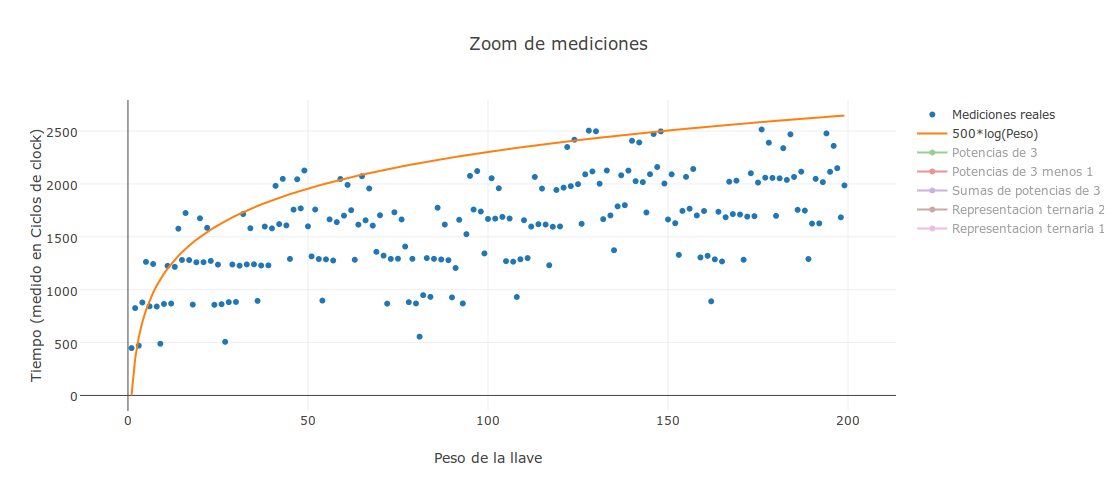
\includegraphics[width=0.8\textwidth]{punto2-zoom}
\caption{Mediciones de la implementaci\'on comparado con $500*log_{3}{n}$ zoom en escala logaritmica en X e Y }
\end{figure}
Si bien se organizaban como líneas rectas (a pesar de la escala), no se acomodaba su $"orden"$ respecto al logaritmo en base 3.
Concluímos que esto se debe a la operación ´´meter la pesa en una balanza", que en la implentación del problema se traduce a introducir un entero al final de una lista, lo cual termina costando $\mathcal{O}(1)$

Para ver si esto era cierto, hicimos nuevas mediciones, tomando para los pesos  solo 3 casos: \\
-Potencias de 3: Que en la representacion ternaria, contaría solo con un 1 y puros ceros \\
-Potencias de 3 menos 1:Que en la representacion ternaria, contaría con todos 2\\
-Suma de potencias de 3:Que en la representacion ternaria, contaría con todos 1\\

y como resultado del experimento nos quedó este gráfico
\begin{figure}[H]
\centering
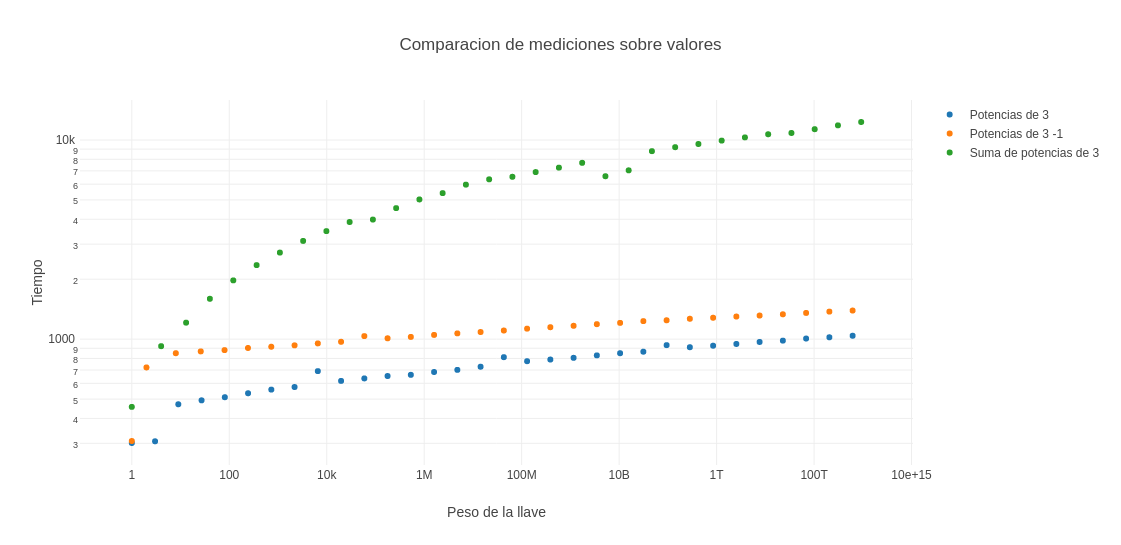
\includegraphics[width=0.4\textwidth]{punto2-comparaciones}
\caption{Comparaciones de la implementaci\'on comparando los casos en escala logarítmica en X e Y }
\end{figure}

En la imagen se puede notar que el caso de suma de potencias de 3 toma mucho más que los otros dos casos. Concluímos que esto se debe incialmente a que, en el caso de sólo potencias de 3, se hace un sólo acceso a la listar, mientras que el caso de potencias de 3 menos 1
tal como sería el resultado al problema, se pone una pesa de la potencia de 3 del lado de la llave y una pesa de tamaño 1 en el otro, teniendo así sólo 2 accesos a la lista, cosa que en la implementación esto se representa sumándole 1 luego de cada división por 3 al peso de la llave en cada iteración.

Como conclusión final a tomar en cuenta, consideramos que los mejores casos son los de potencias de 3 y los peores son los de sumas de potencias de 3.





%%%%%%%%%%%%%%%%%%%%%%%%%%%%%%%%%%%%%%%%%%%%%%%%%%%%%%%%%%%%%%%%%%%%%%%%%%%%%%%%%%%%%%%%%%%%%

\section{Problema 3: Guardando el tesoro}

\subsection{Introducción}

En este problema, los exploradores se encuentran frente a muchos tesoros que desearían poder llevarse. Para esto, cuentan con varias mochilas, cada una con una determinada capacidad de peso que puede cargar.
Los tesoros son de distintos tipos, y cada tipo tiene un peso y un valor determinado.
El objetivo es encontrar la manera óptima de llenar las mochilas para poder llevar el mayor valor posible.

Formalmente, tenemos un conjunto de elementos que tienen como propiedad dos naturales asociados (el peso y el valor). Entonces podemos inferir que existen dos criterios de ordenamiento asociados respectivamente a estos valores.
Al mismo tiempo tenemos otro conjunto de elementos que posee como propiedad un natural asociado (capacidad).
Nuestro objetivo es seleccionar una combinación de los primeros objetos, restringida por las capacidades dadas, de modo de maximizar la sumatoria del valor de los mismos.


\subsection{Explicación de la solución}

   Inicialmente creímos que este problema podría resolverse mediante un algoritmo de BackTracking, sin embargo observamos que nunca lograríamos conseguir la complejidad pedida, puesto que este tipo de algoritmos conlleva una complejidad exponencial superior.
   Finalmente, pudimos resolverlo mediante programación dinámica. Nuestro problema se divide en dos subproblemas:
   Encontrar el valor óptimo, y luego llenar las mochilas con los objetos correspondientes.

   Para obtener el valor óptimo, modelamos nuestro problema a partir de la siguiente función recursiva:

	$f(0,p_{1},p_{2},p_{3})=0 \\
	f(n,p_{1},p_{2},p_{3}) = Max(V_{n}+Max(f(n-1,p_{1}-p_{n},p_{2},p_{3}), f(n-1,p_{1},p_{2}-p_{n},p_{3}), f(n-1,p_{1},p_{2},p_{3}-p_{n})),f(n-1,p_{1},p_{2},p_{3})) $

	Donde n representa el número de tesoro, $V_{n}$ y $P_{n}$ su valor y su peso respectivamente. $p_{1},p_{2}\ y \ p_{3}$ son las capacidades de cada mochila.

<<<<<<< HEAD
	Esta función es del tipo top down, es decir, que para calcular su i-esimo término requiere de los anteriores. En cada estado decide recurivamente sí el mejor valor posible se obtiene de sólo guardar nuestro i-esimo objeto o en alguna de las tres mochilas, o en ninguna mochila.
=======
	Esta función,al ser recursiva, para calcular su i-esimo término requiere de los anteriores. En cada estado decide recurivamente sí el mejor valor posible se obtiene de sólo guardar nuestro i-esimo objeto o en alguna de las tres mochilas, o en ninguna mochila.  
>>>>>>> 07e1e05216c3d0cd0569c50823acb3bc96dfe0d3



	Para resolver nuestro primer problema el algoritmo se encarga de llenar un arreglo de cuatro dimensiones, donde el tamaño del arreglo principal es la cantidad de objetos y los tamaños de los otros tres arreglos anidados son las capacidades de las tres mochilas.
	Lo que representa cada posición, (x,y,z,w), de este arreglo es el valor óptimo que pueden lograr los primeros x objetos con una combinación de mochilas de peso y, z, w. En el caso que el problema a resolver responda a dos mochilas, una de las variables y, z, w seran 0 para cualquier posción y un caso similar si solo hay que llenar una mochila.

<<<<<<< HEAD
%%%%%%%TERMINA MODIFICACION%%%%
	Luego para llenar las mochilas utilizamos este arreglo (lleno luego de encontrar el valor ótimo) entonces para cada objeto i guardamos el valor óptimo es decir, la posición del arreglo (i,cap1,cap2,cap3). Después nos fijamos para cada mochila  el resultado de sumar el valor del objeto i con el valor óptimo para el objeto anterior menos el valor óptimo guardado, si esto da cero, es porque encontramos la mochila a la cual corresponde el objeto i.
=======
>>>>>>> 07e1e05216c3d0cd0569c50823acb3bc96dfe0d3

	Luego para llenar las mochilas utilizamos este arreglo (lleno luego de encontrar el valor ótimo) entonces para cada objeto i guardamos el valor óptimo es decir, la posición del arreglo (i,cap1,cap2,cap3). 

	Después para decidir en cuál mochila tendría que ser guardado revisamos la posición que corresponde al objeto anterior (i-1) y para cada mochila, las otras tres coordenadas serán, la capacidad de la mochila que estamos revisando menos el peso del objeto i, y las otras dos se mantienen constantes. Si esto da cero, es porque encontramos la mochila a la cual corresponde el objeto i, si no ese objeto no debe ser metido en ninguna mochila. 


	Observación: nuestro algoritmo descarta los tesoros que tienen un peso mayor al máximo de capacidad entre las mochilas. Asumimos en el pseusocódigo que nuestra entrada cumple esa propiedad.


\subsubsection{Pseudocódigo}

\begin{algorithm}[H]{\textbf{guardandoTesoro}(mochilas: vector$<$mochila$>$, cofre: vector$<$tesoro$>$)}
	\begin{algorithmic}[1]
		%\State objXpesos $\gets$ Hipercubo() incializado en -1 \Comment (en las posiciones donde no puede haber objetos incializo en 0) %$\mathcal{O}$()
		\State objXpesos $\gets$ 4-upla donde con todos los valores son -1 excepto en las posiciones donde no puede haber objetos que valen  0 %$\mathcal{O}$()
		\State sol$\gets$ ValorOptimo(objXpesos,cofre,cofre.size-1,capacidades de las mochilas)
		\State LlenarMochilas(objXpesos, cofre, mochila1, mochila2, mochila3)
		\State return (sol, mochilas)
	\end{algorithmic}
\end{algorithm}



\begin{algorithm}[H]{\textbf{LlenarMochilas}(objetoXpeso: hipercubo, cofre:vector$<$tesoro$>$, m1,m2,m3:mochilas)}
	\begin{algorithmic}[1]
		\State desde i= cofre.size-1 hasta i=0
			\State \quad obj $\gets$ cofre[i]
			\State \quad cap1 $\gets$ m1.Capacidad
			\State \quad cap2 $\gets$ m2.Capacidad
			\State \quad cap3 $\gets$ m3.Capacidad
			\State \quad Si $i=0$ hacer
				\State \quad \quad Agregar obj en cualquier mochila en la que entre.
			\State \quad Si no hacer
				\State \quad \quad valM1 $\gets$ obj.valor + ValorOptimo(objetoXPeso, cofre, i,cap1-obj.peso,cap2,cap3 )
				\State \quad \quad valM2 $\gets$ obj.valor + ValorOptimo(objetoXPeso, cofre,i,cap1,cap2-obj.peso,cap3 )
				\State \quad \quad valM3 $\gets$ obj.valor + ValorOptimo(objetoXPeso, cofre,i, cap1, cap2,cap3-obj.peso )
				\State \quad \quad  MeterEnCorrecta(valM1,valM2,valM3,m1,m2,m3,obj)
			\State \quad finSi

	\end{algorithmic}
\end{algorithm}



%%%

\begin{algorithm}[H]{\textbf{ValorOptimo(objXpeso:4-upla, cofre:vector$<$tesoro$>$, objeto:int, peso1: int, peso2:int, peso3:int)}}
	\begin{algorithmic}[1]
		\State  pesoObj $\gets$ cofre[objeto].peso
		\State  pesoVal $\gets$ cofre[objeto].valor

		\State Si $peso1 < 0 \vee peso2 < 0 \vee peso3 < 0$
			\State \quad devolver $-1$

		\State finSi

		\State Si objetoxPesos[objeto][peso1][peso2][peso3] $\neq$ -1
			\State \quad devolver objetoxPesos[objeto][peso1][peso2][peso3]
		\State finSi
		\State Si objeto $=$ 0
			\State \quad val $\gets$ 0

			\State \quad Si peso1 $\ge$ pesoObj $\vee$ peso2 $\ge$ pesoObj $\vee$ peso3 $\ge$ pesoObj
				\State\quad \quad  val $\gets$ valorObj

				\State \quad \quad objetoxPesos[objeto][peso1][peso2][peso3] $\gets$ val
				\State \quad \quad devolver val
			\State \quad Si no
				\State \quad \quad devolver -1 %esta bien?%
			\State \quad finSi

		\State Si no
			\State \quad PosiblesSolus $\gets$ vector$<$int$>$
			\State \quad sinObj $\gets$ ValorOptimo(objetoxPesos, cofre, objeto -1, peso1, peso2, peso3)
			\State \quad PosiblesSolus.Agregar(sinObj)
			\State \quad Desde j=1 hasta j=3 hacer
				\State \quad \quad Si pesoj-pesoObj $\ge$ 0
					\State \quad \quad \quad objenj $=$ valorObj + ValorOptimo(objetoxPesos, cofre, objeto - 1, pesoj - pesoObj, los otros dos pesos)
					\State \quad \quad \quad PosiblesSolus.Agrergar(objenj)
				\State \quad \quad finSi
			\State \quad finDesde
			\State \quad  valor$\gets$Max(PosiblesSolus)
			\State \quad objetoxPesos[objeto][peso1][peso2][peso3] $\gets$ valor
			\State \quad return valor
		\EndIf


	\end{algorithmic}
\end{algorithm}

\newpage

\subsubsection{Demostración de Correctitud}
Presentaremos la función matemática que modela nuestro problema:\\ %cambiar%

$f(o,p_{1},p_{2},p_{3})=0 \\
f(n,p_{1},p_{2},p_{3}) = Max(V_{n}+Max(f(n-1,p_{1}-p_{n},p_{2},p_{3}), f(n-1,p_{1},p_{2}-p_{n},p_{3}), f(n-1,p_{1},p_{2},p_{3}-p_{n})),f(n-1,p_{1},p_{2},p_{3})) $
\\
Donde n representa el número de tesoro, $V_{n}$ y $P_{n}$ su valor y su peso respectivamente. $p_{1},p_{2}\ y \ p_{3}$ son las capacidades de cada mochila.

Para la demostración utilizaremos inducción global en n.
\\
\\
Caso base: queremos ver que $f(0,p_{1},p_{2},p_{3})$ resulta ser el valor máximo que se puede obtener con 0 objetos:
$f(0,p_{1},p_{2},p_{3}) = 0$ al tener 0 objetos el valor de los mismos es 0 de modo que es el máximo valor posible.
\\
\\
Hipótesis Inductiva: $\forall k<n$ vale que $f(k,p_{1},p_{2},p_{3})$ da el valor máximo que se puede obtener con k objetos.
\\
\\
Ahora queremos ver que $f(n,p_{1},p_{2},p_{3})$ da el valor óptimo para n objetos.
\\
\\
$f(n,p_{1},p_{2},p_{3}) = Max(V_{n}+Max(f(n-1,p_{1}-p_{n},p_{2},p_{3}), f(n-1,p_{1},p_{2}-p_{n},p_{3}), f(n-1,p_{1},p_{2},p_{3}-p_{n})),f(n-1,p_{1},p_{2},p_{3})) $ \\
por hipótesis inductiva (como $n-1 \leq k$ para algun k) sabemos que $f(n-1,p_{1}-p_{n},p_{2},p_{3}), f(n-1,p_{1},p_{2}-p_{n},p_{3}), f(n-1,p_{1},p_{2},p_{3}-p_{n}) y f(n-1,p_{1},p_{2},p_{3})$ son los valores óptimos que se pueden conseguir con n-1 objetos restando (o no) el peso del objeto n de modo de luego poder guardarlo en alguna mochila (o no). Utilizaremos los renombres $V_{01},V_{02},V_{03},V_{00}$ respectivamente.
Entonces tenemos: \\
$f(n,p_{1},p_{2},p_{3})= Max(V_{n}+Max(V_{01},V_{02},V_{03}),V_{00})$\\
Podemos ver que esta función  compara el valor óptimo de llenar las mochilas con n-1 tesoros y el tesoro n, con el valor óptimo de llenar las mochilas con n-1 tesoros sin el tesoro n (de esta forma se tiene cuenta el caso en el que el mejor valor se obtiene de poner algún objeto  de los n-1 anteriores que impide luego meter el tesoro n).\\
Como la función Max devuelve el mayor valor, el resultado sera el óptimo.
\\
Como valen P(0)..p(k) $\forall k<n$ y vale p(n) $\Rigtharrow$ vale p(n) $\forall n \in N \cup {0} $

En nuestra demostración utilizamos el principio de optimalidad. Ahora probaremos que efectivamente queremos construir nuestra solución a partir de subsoluciones óptimas:

Supongamos que $f(n,p_{1},p_{2},p_{3}) = Max(V_{n} + H, V_{00})$ donde H es una subsolución del estado anterior que no es óptima. sabemos que $ H < Max(V_{01},V_{02},V_{03})$ (ya que si no sería óptima) entonces $V_{n}+H < V_{n}+Max(V_{01},V_{02},V_{03})$ (ya que estamos sumando números positivos) Luego $Max(V_{n}+H,V_{00}) \leq Max(V_{n}+Max(V_{01},V_{02},V_{03}), V_{00})$ entonces $f(n,p_{1},p_{2},p_{3})$ no es óptimo, absurdo. 



\subsubsection{Demostración de Complejidad}

La complejidad del algoritmo GuardarTesoro es $\mathcal{O}(\prod_{i=1}^{3}K_{i} * T)$ donde $K_i$ representa la capacidad de cada mochila y T la cantidad de tesoros. Además, esta complejidad es aportada por el algoritmo ValorOptimo, entonces basaremos nuestra demostración en el mismo.

Primero haremos unas observaciones preliminares:
\begin{itemize}
%%modificacion
	\item Se puede pensar que el arreglo de cuatro dimensiones en realidad es un arreglo de cubos, donde el índice de cada cubo es hasta que objeto se verifico la solución optima. 
%%%finModif
	\item El volumen de un cubo es es $\prod_{i=1}^{3}A_{i}$ donde cada $A_i$ es una arista que representa el eje de la altura, el ancho o el largo. En este caso las aristas de los cubos serán las capacidades de las mochilas, sabemos que llenar una posición del cubo nos cuesta $\Theta(1)$, entonces llenarlo entero nos costará el equivalente al volumen del mismo.
	\item Llenar un hipercubo, o arreglo de cubos, con un valor determinado (como ocurre en la linea 1 de guardandoTesoro) cuesta $\mathcal{O}(\prod_{i=1}^{3}K_{i} * T)$ ya que hay T cubos para llenar.
	\item Cuando se llama a LlenarMochilas desde GuardarTesoro cuesta $\Theta{O}(T)$ ya que en en las lineas 9,10,11 cuando se llama a ValorOptimo, el hipercubo objetoXpeso cuenta con todos lo valores ya calculados entrando en el if (linea 6) que devuelve en $\Theta(1)$ el valor.
\end{itemize}

Volviendo a la demostración, tanto en el pseudocódigo como en la función matemática podemos ver que la recursión se realiza a lo sumo cuatro veces la cantidad total de tesoros, pero estas recursiones se hacen sobre valores distintos, posiciones distintas del arreglo y referenciamos al hipercubo. Para llenar un cubo, siempre debemos recurrir al cubo anterior, uno puede pensar que esto aportaría complejidad, sin embargo, al guardar estos valores sólo construimos estos cubos una vez, y la complejidad por acceso es $\Theta(1)$.

como se guardan los valores y en ninguna recursividad  el algoritmo recalcula un valor, la complejidad está dada por llenar el arreglo de cubos. Concluyendo que la complejidad es $\mathcal{O}(\prod_{i=1}^{3}K_{i} * T)$

Ahora probemos que esta complejidad es menor a la pedida ($\mathcal{O}((\sum_{i=1}^{3}K_{i})^{3} * T)$)
\\
quiero ver que $\mathcal{O}(\prod_{i=1}^{3}K_{i} * T)$ $\leq$ $\mathcal{O}((\sum_{i=1}^{3}K_{i})^{3} * T)$
\\
si T es cero la desigualdad es verdadera,sino es equivalente probar que $\mathcal{O}(\prod_{i=1}^{3}K_{i})$ $\leq$ $\mathcal{O}((\sum_{i=1}^{3}K_{i})^{3})$
\\
Si expandimos la suma y la productoria nos queda :
\\
K_1*K_2*K_3 $\leq$ K_1^3+K_2^3+K_3^3 +3*K_1^2*K_2 + 3*K_1^2*K_3 + 3*K_2^2*K_1 + 3*K_2^2*K_3 +3*K_3^2*K_1 + 3*K_3^2*K_2 + 6*K_1*K_2*K_3.
\\
0 $\leq$ K_1^3+K_2^3+K_3^3 +3*K_1^2*K_2 + 3*K_1^2*K_3 + 3*K_2^2*K_1 + 3*K_2^2*K_3 +3*K_3^2*K_1 + 3*K_3^2*K_2 + 6*K_1*K_2*K_3.
\\
como K_i $\geq$ 0 para todo i, eso se cumple y demostramos que la complejidad es menor a la pedida.


\subsection{Experimentación}

La cota de complejidad de nuestro algoritmo es $\prod_{i=1}^{3}K_{i}* T$. Es decir que depende de la capacidad y cantidad de mochilas y la cantidad de tesoros.
En esta sección trataremos de respaldar esta cota mediante el análisis de los datos empíricos que obtuvimos a traves del testeo de nuestro algoritmo.
Con este objetivo a lo largo de los tests modificamos los inputs para observar de a una variable por vez dejando las otras constantes y así poder analizar el tiempo de ejecución en cada caso. En cada test los valores se logran al promediar tres mil iteraciones sobre el mismo input, sobre que forma tiene el input se va a hablar más adelante.
%%%%MODIFICACION "EN cada test... hablar mas adelante."

\subsubsection{Resultados y análisis}

En nuestro primer experimento fijamos una mochila con capacidad constante (50) y fuimos aumentando la cantidad de tesoros de a dos.
Así mismo, analizamos tres subcasos pertinentes: cuando los objetos están dados aleatoriamente (sin ninguna restricción sobre su peso), cuando el peso de los objetos se encuentra restringido a la capacidad de la mochila y cuando el peso de objetos es superior a la capacidad de la mochila.

\begin{figure}[H]
\centering
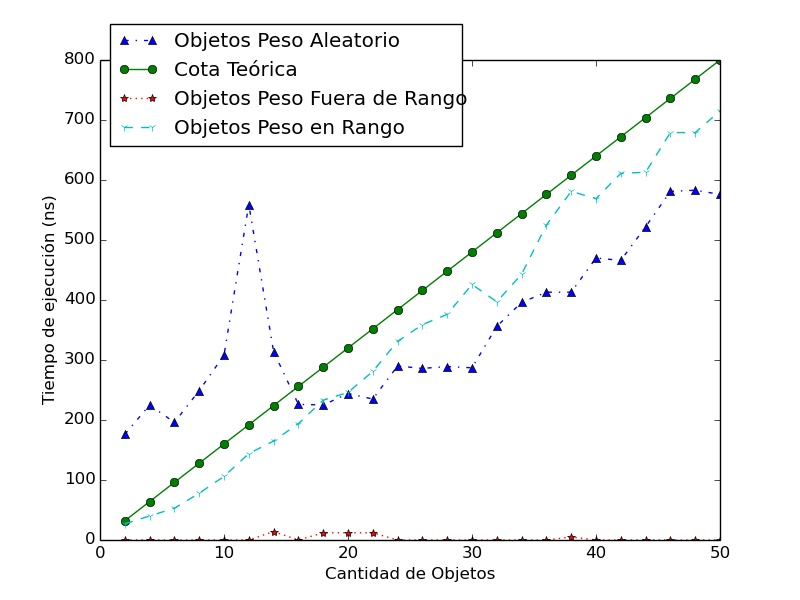
\includegraphics[width=0.6\textwidth]{ObjMejorCasoVsAbjRangovsObjAl}
\caption{gráfico comparativo de los tres subcasos al variar T.}
\end{figure}


En esta figura podemos observar no solo la tendencia lineal en la complejidad del algoritmo sino también la variación del crecimiento del tiempo para los distintos casos.
El hecho de que los gráficos sean lineales respaldan nuestra cota de complejidad ya que estaríamos variando el parámetro T mientras $K_1$ (la capacidad de la mochila) se mantiene constante. Estaríamos bajo la presencia de una función de tipo $Y=c*X$ con c constante.
En particular podemos destacar que en el caso de que los objetos tengan todos peso mayor a la capacidad de las mochilas, la recta tiende a ser constante y el tiempo de ejecución es casi nulo.
Podemos concluir que este sería nuestro mejor caso, y se debe al hecho de que filtramos nuestra entrada para que no se tengan en cuenta estos tesoros.
Tambien se puede observar una sección donde los objetos con peso aleatorio tienen un tiempo de ejecución que los otros casos, esto bien puede resultar de los valores de los pesos. Si los pesos en son menores en el caso de los pesos aleatorios a los pesos en rango, la cantidad de recursiones a las que se lllama, son mayores. 
Observemos que en general lleva más tiempo obtener un resultado cuando los objetos tienen peso menor a la capacidad de la mochila.

\\
\\
\\
Luego realizamos tests para poder ver el comportamiento del algoritmo al ir aumentando el peso de la mochila. Utilizamos un test para evaluar el comportamiento cuando los objetos son aleatorios y otro para cuando todos los tesoros tienen un peso mayor a la capacidad de la mochila, en ambos casos la cantidad de objetos es constante en 50 elementos.
En esta figura podemos observar no solo la tendencia lineal de la complejidad del algoritmo sino también la variación de las pendientes en cada caso. Notemos que a mayor pendiente, la ejecución toma más tiempo, es decir es ´´más lenta".
En particular podemos destacar que en el caso de que los objetos tengan todos peso mayor a la capacidad de las mochilas, la recta tiende a ser constante.

\begin{figure}[H]
\centering
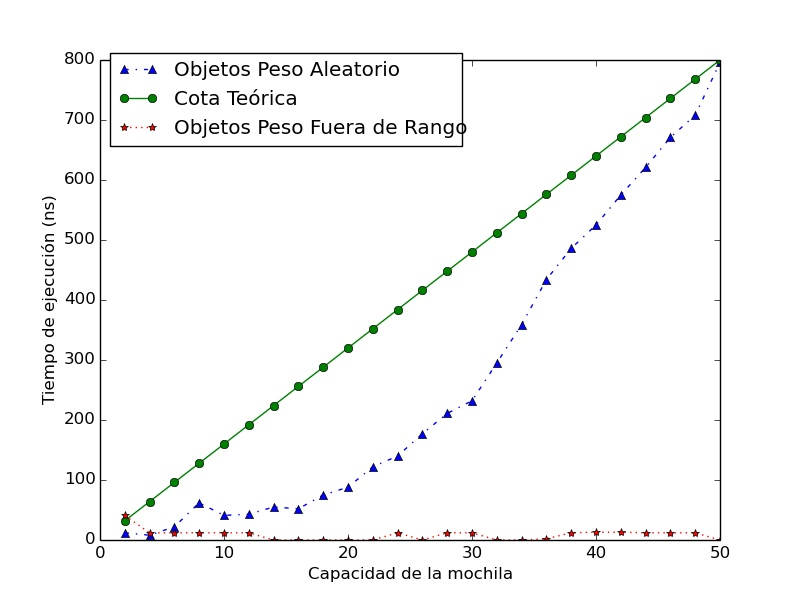
\includegraphics[width=0.6\textwidth]{ObjMejorCasoPesovsPesoDistSL}
\caption{gráfico comparativo al variar K}
\end{figure}

Podemos observar que al tener los tesoros con peso fuera del rango de la capacidad de la mochila el tiempo se mantiene constante, prácticamente nulo igual que en el experimento anterior. Con los objetos aleatorios vemos que tiene cierta tendencia lineal como es de esperarse (ya que este caso es similar al analizando en la figura()) sin embargo algunos valores quedan distorcionados. Creemos que esto se debe a que los objetos son aleatorios.
\\
\\
Finalmente corrimos tests variando la cantidad de mochilas (todas con capacidad 50) manteniendo constantes los tesoros, estos siendo 50. Este gráfico va a tener escala logaritmica en el eje y para poder observar su comportamiento exponencial.
\\
\\
En el  gráfico se trata de comparar como afecta la distribución de pesos en las mochilas. Como nuestra complejidad varía dependiendo del producto de las capacidades queríamos ver como era el tiempo de ejecución para distinta cantidad de mochilas con el mismo producto. tomamos cincuenta objetos con peso igual a la capacidad mínima del conjunto de mochilas en el que testeamos y repetimos cada instancia mil veces tomando el promedio.
\begin{figure}[H]
\centering
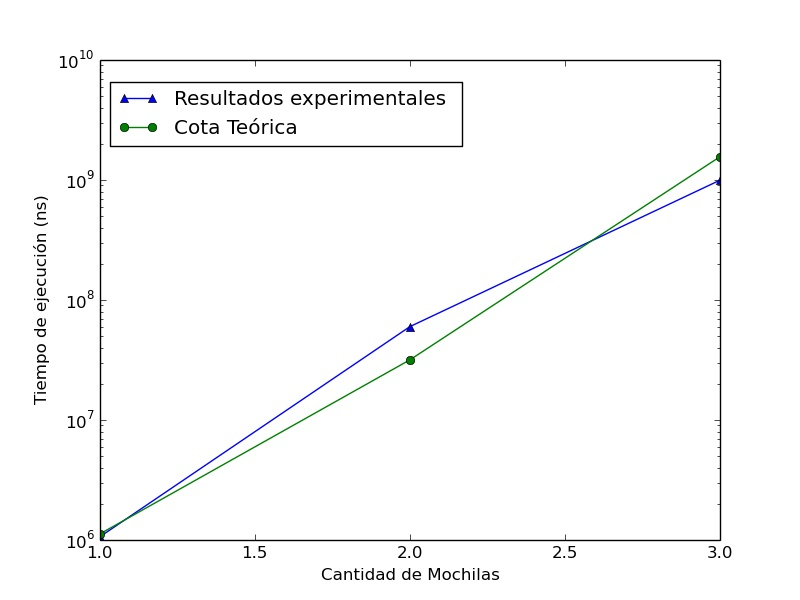
\includegraphics[width=0.6\textwidth]{VariaMoch}
\caption{variación de la cantidad de mochilas.}
\end{figure}

En esta figura podemos observar el crecimiento exponencial del tiempo dependiendo de la cantidad de mochilas, como la escala es logaritmica y las curvas son casi lineas rectas entonces podemos deducir que el tiempo crece de forma exponencial. Esto concuerda con el hecho de que al tener todas las variables en 50 ($T=50, K_1 =50 k_2=50, k_3=50$) al ir aumentando la cantidad de mochilas estaríamos elevando la constante 50 (con $K_1$ tenemos $K_1*T=50^2$, con $K_2$ tenemos $K_1*K_2*T=50^3, etc $). Este es el tipo de función exponencial $Y=50^X$.
\\
\\
En el último gráfico se trata de comparar como afecta la distribución de pesos en las mochilas. Como nuestra complejidad varía dependiendo del producto de las capacidades queríamos ver como era el tiempo de ejecución para distinta cantidad de mochilas con el mismo producto. tomamos cincuenta objetos con peso igual a la capacidad mínima del conjunto de mochilas en el que testeamos y repetimos cada instancia mil veces tomando el promedio. 
\begin{figure}[H]
\centering
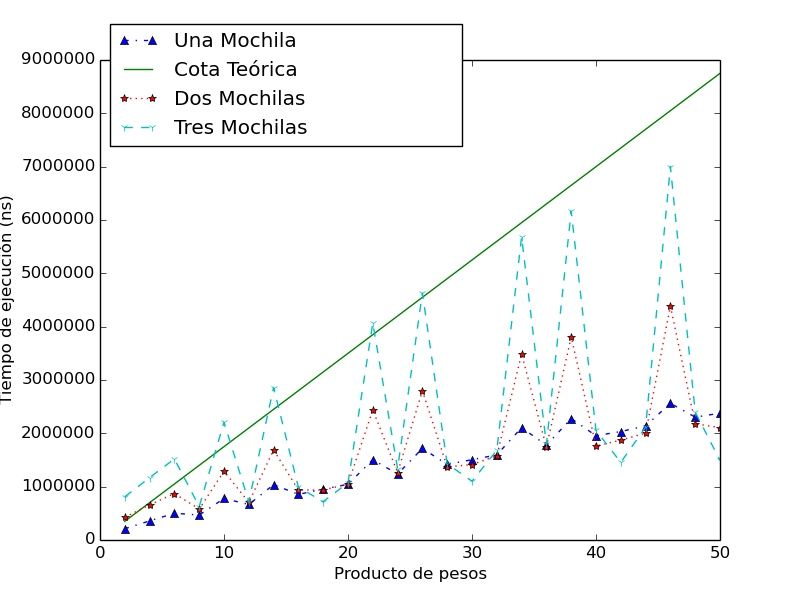
\includegraphics[width=0.8\textwidth]{MismoPesoCompRang}
\caption{variación de la Productaria de Pesos.}
\end{figure}
\\
En el gráfico separaremos las mediciones en 3 partes, una los picos altos, desde el seis y cada cuatro números con la excepción de cuatro casos. Dos los picos bajos desde el ocho y cada cuatro números y tres, las anomalías que rompen el patrón de los picos altos. Debajo pondremos cuales son las capacidades, en cada tabla especificamos si ese peso responde a Picos Altos, Bajos o anomalías.
\\


\begin{center}
 \begin{tabular}{|c |c |c|||c|c|c|} 
 \hline
 Picos Altos & Dos mochilas & Tres mochilas&Picos Altos & Dos mochilas & Tres mochilas\\ [0.5ex] 
 \hline\hline
 2 & 1*2 & 1*1*2 & 8 & 2*4 & 2*2*2 \\ 
 \hline
 4 & 2*2 & 1*2*2 & 12 & 3*4 & 2*2*3\\
 \hline
 6 & 2*3 & 1*2*3 & 16 & 4*4 & 2*2*4\\
 \hline
 10 & 2*5 & 1*2*5 & 20 & 4*5 & 2*2*5 \\
 \hline
 14 & 2*7 & 1*2*7 & 24 & 4*6 & 2*2*6 \\
 \hline
 22 & 2*11 & 1*2*11 & 28 & 4*7 & 2*2*7\\
 \hline
 26 & 2*13 & 1*2*13 & 32 & 4*8 & 2*2*8\\
 \hline
 34 & 2*17 & 1*2*17 & 36 & 6*6 & 2*2*9\\
 \hline
 38 & 2*19 & 1*2*19 & 40 & 8*5 & 2*2*10\\
 \hline
 46 & 2*23 & 1*2*23 & 44 & 11*4 & 2*2*11\\  
 \hline
- & - & - & 48 & 8*6 & 2*2*12\\ [1ex] 
 \hline
\end{tabular}
\end{center}



\begin{center}
 \begin{tabular}{|c | c | c|} 
 \hline
 Anomalías & Dos mochilas & Tres mochilas  \\ [0.5ex] 
 \hline\hline
 18 & 3*6 & 2*3*3  \\ 
 \hline
 30 & 5*6 & 2*3*5 \\
 \hline
 42 & 6*7 & 2*3*7 \\
 \hline
 50 & 5*10 & 2*5*5  \\ [1ex] 
 \hline
\end{tabular}
\end{center}




\\
En los picos altos la cantidad de mochilas importa, en el mismo producto de pesos 3 mochilas tardan más que 2 y las dos tardan más que 1 sola. Lo cual por la complejidad teórica resulta incoherente, aún así, esto se puede explicar por como creamos las pruebas. En los picos altos los pesos de los objetos es uno, esto quiere decir que no solo todos los objetos entran, sino que los pesos de las mochilas se reducen de a uno, lo cual genera mayores llamadas a las recursiones. si es una sola mochila hace dos llamadas, si son tres hace cuatro y esto depende directamente de los pesos, si los pesos fueran mas grande, algunas llamadas recusivas no las haría por que se irían de rango.
\\
\quad En cambio en los picos bajos se puede ver como se reducen los pesos de una forma más rápida ya que los pesos son dos, haciendo menos llamadas recursivas.
\\
\quad Ahora nos falta hablar de los cuatro elementos que no solo rompen con el patrón de los picos altos, sino que tambien a diferencia de los picos bajos hace que los tiempo de ejecución de tres mochilas sean menos que el de dos o el de una. Esto se explica tambien con los pesos que se eligieron para llenar las mochilas, sigue siendo dos, pero en este caso entra menos veces a las llamadas en compuesto por tres ya que los pesos de cada mochila es menor.
\\
\quad En conclusión podemos decir que los tiempos de ejecución, si decidimos que los objetos tengan como peso mínimo la capacidad mínima del conjunto de mochilas, tardan menos que cuanto más homogénea sea la descomposición, hasta favoreciendo el caso de más mochilas, y cuanto más desbalanceada sea la descomposición más va a tardar, favoreciendo el caso de menos mochilas. Entonces podemos decir que tenemos números que sus productos son más valiosos en tiempo de ejecución que otros, por ejemplo sabemos que los primos van a tardar notablemente más si son más mochilas y tambien podemos suponer con cierto grado de certeza que los cubos perfectos son más eficientes en tiempo si decidímos dividirlo en tres mochilas.
\\
\\




:-"Y todos estos tesoros van a ir para algun museo no?"
\\
:-"Sí,Indi... lo que digas..."



\end{document}
